\chapter{The LHCb Experiment}
\label{ch:lhcb}

The Large Hadron Collider beauty (LHCb) experiment \cite{lhcb2008, lhcb2015} is one of the four main experiments at the Large Hadron Collider (LHC) \cite{lhc_machine2008} at the European Organization for Nuclear Research (CERN), which is located in Geneva, Switzerland. It is designed to study the properties of beauty and charm hadrons, with a primary focus on precision measurements of rare decays, CP violation, spectroscopy, and the search for NP.

At CERN, protons are accelerated to ultra-relativistic speeds through a complex of accelerators. The last stage in the acceleration chain is the LHC, a synchrotron particle collider situated $\qty{100}{\meter}$ underground, with a circumference of $\qty{26.7}{\kilo\meter}$. In the LHC, two proton beams are accelerated in opposite directions and made to collide at four interaction points, reaching a center-of-mass energy of $\sqrt{s} =  \qty{13}{\tera\electronvolt}$ during Run 2 and $\sqrt{s} = \qty{13.6}{\tera\electronvolt}$ in Run 3 of the LHC. Superconducting dipole magnets guide the particles around the ring, while quadrupole magnets focus them into tight beams. The acceleration is achieved using radio-frequency cavities.

The LHCb detector is located at the intersection point 8 of the LHC ring and is designed as a single-arm forward spectrometer, optimized for the predominantly forward and backward production of beauty and charm hadrons in $pp$ collisions. The following sections describe the LHCb detector in its Run 2 and Run 3 configurations, with a focus on the changes introduced by the upgrade for Run 3.

\section{Run 2}
\label{sec:lhcb_run2}
Run 2 of the LHC took place from 2015 to 2018. \cref{fig:lhcb_run2} shows a schematic overview of the LHCb detector during this data-taking period. The detector is composed of several subdetectors that can be grouped into two types of systems. The tracking system comprises the Vertex Locator (VELO), a dipole magnet, the Tracker Turicensis (TT), and three downstream tracking stations (T1, T2, and T3). The particle identification system includes the Ring Imaging Cherenkov (RICH) detectors, the electromagnetic and hadronic calorimeters (ECAL and HCAL), and the muon system (M1–M5). 
%The muon system additionally provides tracking information for muons.
\begin{figure}
    \centering
    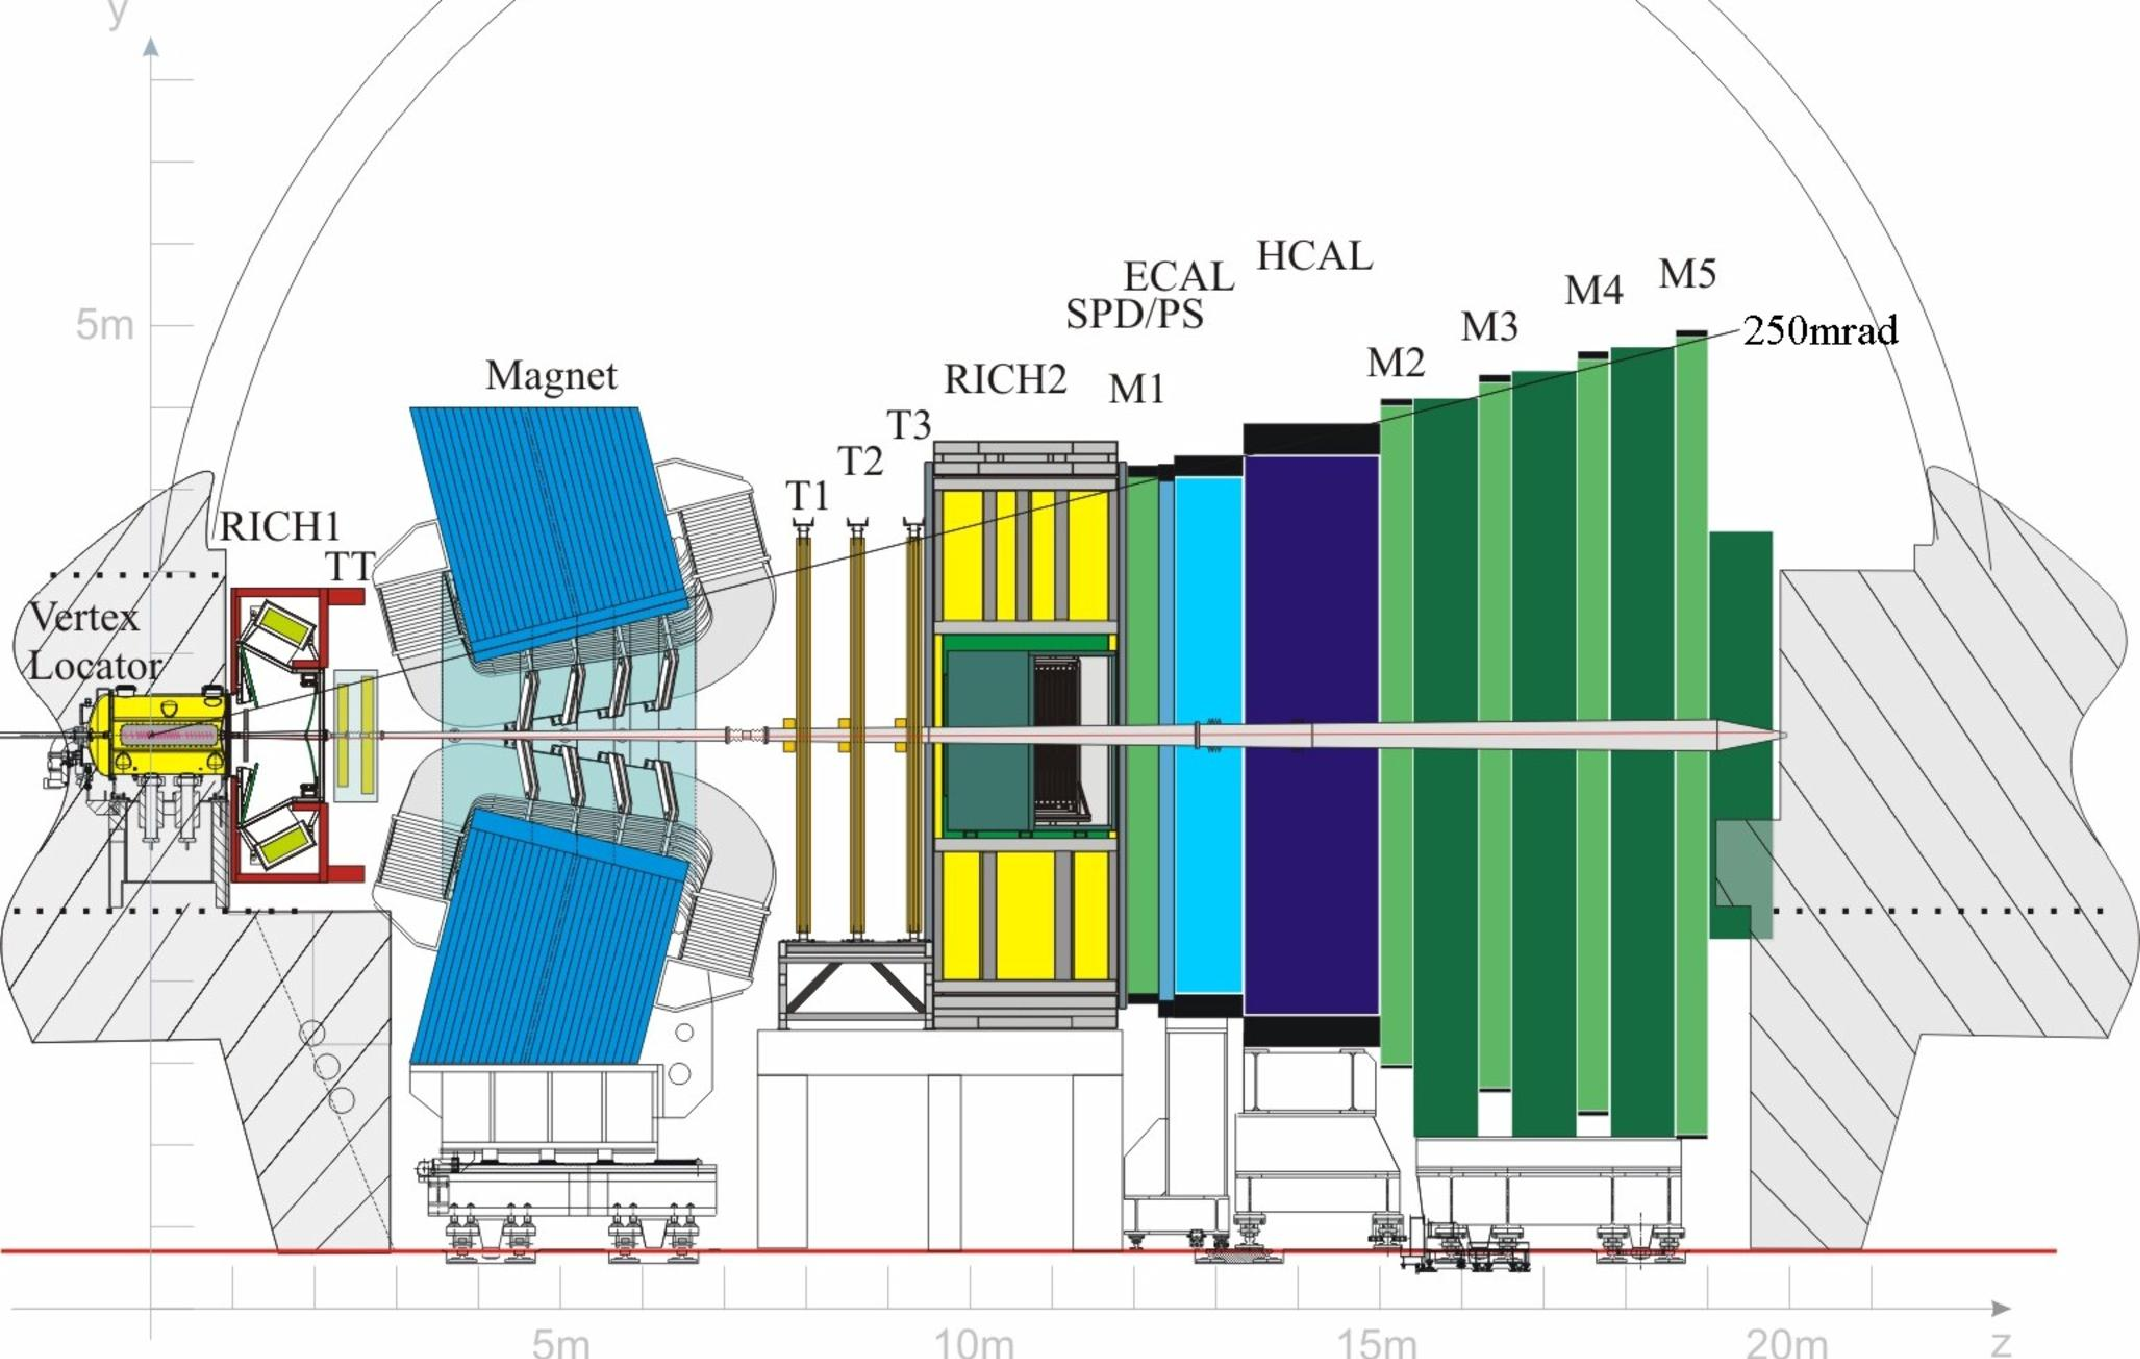
\includegraphics[width=0.9\textwidth]{figures/lhcb_run2.png}
    \caption{Side view of the LHCb detector and its subdetectors during Run 2, taken from \cite{calabrese2022_rich_run2}.}
    \label{fig:lhcb_run2}
\end{figure}

The VELO is a silicon microstrip detector that surrounds the $pp$ interaction region and is used to measure tracks of ionizing particles containing beauty or charm quarks as well as their primary and secondary vertices. The tracking stations and the TT are located behind the VELO and are essential for
the reconstruction of the trajectories of charged particles. T1, T2, and T3 each consist of a silicon microstrip Inner Tracker (IT) and an Outer Tracker (OT), a drift detector based on straw tube technology. The TT, also a silicon microstrip detector, is located between RICH1 and the magnet, whereas T1, T2, and T3 are positioned downstream of the magnet. This arrangement enables the measurement of charged-particle momenta via the bending of their trajectories in the magnetic field. Even in the absence of VELO information, the TT delivers upstream tracking data that is essential for the momentum reconstruction of long-lived particles such as the $\Lambda^0$ hyperon. In order to eliminate systematic effects, the magnet polarity is reversed several times during the year.

The RICH1 detector, located behind the VELO, and the RICH2 detector, located behind T3, are used for particle identification by measuring the Cherenkov radiation emitted by charged particles that travel faster than the speed of light in the detector medium. The angle $\Theta_{\text{c}}$ of the emitted Cherenkov radiation is dependent on the particle's velocity and the refractive index of the medium. The velocity can be expressed through the momentum $p$ and mass $m$ of the particle. This enables testing mass hypotheses using the reconstructed momentum and the measured Cherenkov angle. LHCb employs
two RICH detectors with different radiators to achieve particle identification across a wider momentum range.

The electromagnetic calorimeter (ECAL) and the hadronic calorimeter (HCAL) are located behind RICH2. They are used for energy reconstruction and particle identification. The ECAL intercepts electromagnetically interacting particles, mostly photons and electrons. These particles deposit their energy in the ECAL through electromagnetic showers, which can be used to reconstruct the particle's energy and impact position. The ECAL is made of alternating layers of lead and scintillating material, where the lead acts as an absorber material and the scintillating material as a sensitive medium to detect the electromagnetic showers. Since hadronic showers are larger in their longitudinal expansion than electromagnetic showers, the HCAL is placed behind the ECAL. It is made of iron and scintillating material, and works in a similar way to the ECAL, but is designed to measure the energy of hadrons, such as  pions and protons. In order to aid the particle identification process, the Scintillating Pad Detector (SPD) and Preshower Detector (PS) are placed in front of the ECAL. The SPD allows distinguishing between charged and neutral particles by measuring the scintillation light produced when charged particles pass through scintillator pads. Right behind the SPD, a thin lead converter is placed, followed by the PS. Photons and electrons start an early electromagnetic shower in the lead converter, which is then measured by scintillator pads in the PS, enabling the identification of these particles. 

The muon stations are the last elements of the LHCb detector. Muons are minimum ionizing particles and therefore pass through the calorimeters without losing large amounts of energy. A muon station consists of alternating layers of iron as an absorber and multi-wire proportional chambers, which are used to measure muon tracks. The absorber ensures that only muons reach the detector, enabling the identification of muons.

Within the constraints of the experiment’s technical and storage infrastructure, it is not feasible to record data at the full bunch-crossing rate of the LHC. Since many collisions produce background events of no interest, the LHCb detector employs several trigger systems to select events of potential relevance. The Level 0 trigger (L0) is a hardware trigger that selects events based on the information from the calorimeters and muon system, to filter events with high transverse momenta or energy above a defined threshold. The High Level Trigger (HLT) is the second trigger level and is fully software-based. It is further divided into HLT1, which uses partially reconstructed events, and HLT2, which uses fully reconstructed events, in order to perform the selection.

\section{Run 3}
\label{sec:lhcb_run3}
Run 3 of the LHC began in 2022 and is scheduled to continue until 2026. To enhance its performance and handle an instantaneous luminosity five times higher than in earlier runs, the LHCb detector underwent a major upgrade, referred to as Upgrade I \cite{lhcb_upgrade_I}. \cref{fig:lhcb_run3} presents a schematic overview of the detector following this Upgrade.
\begin{figure}
    \centering
    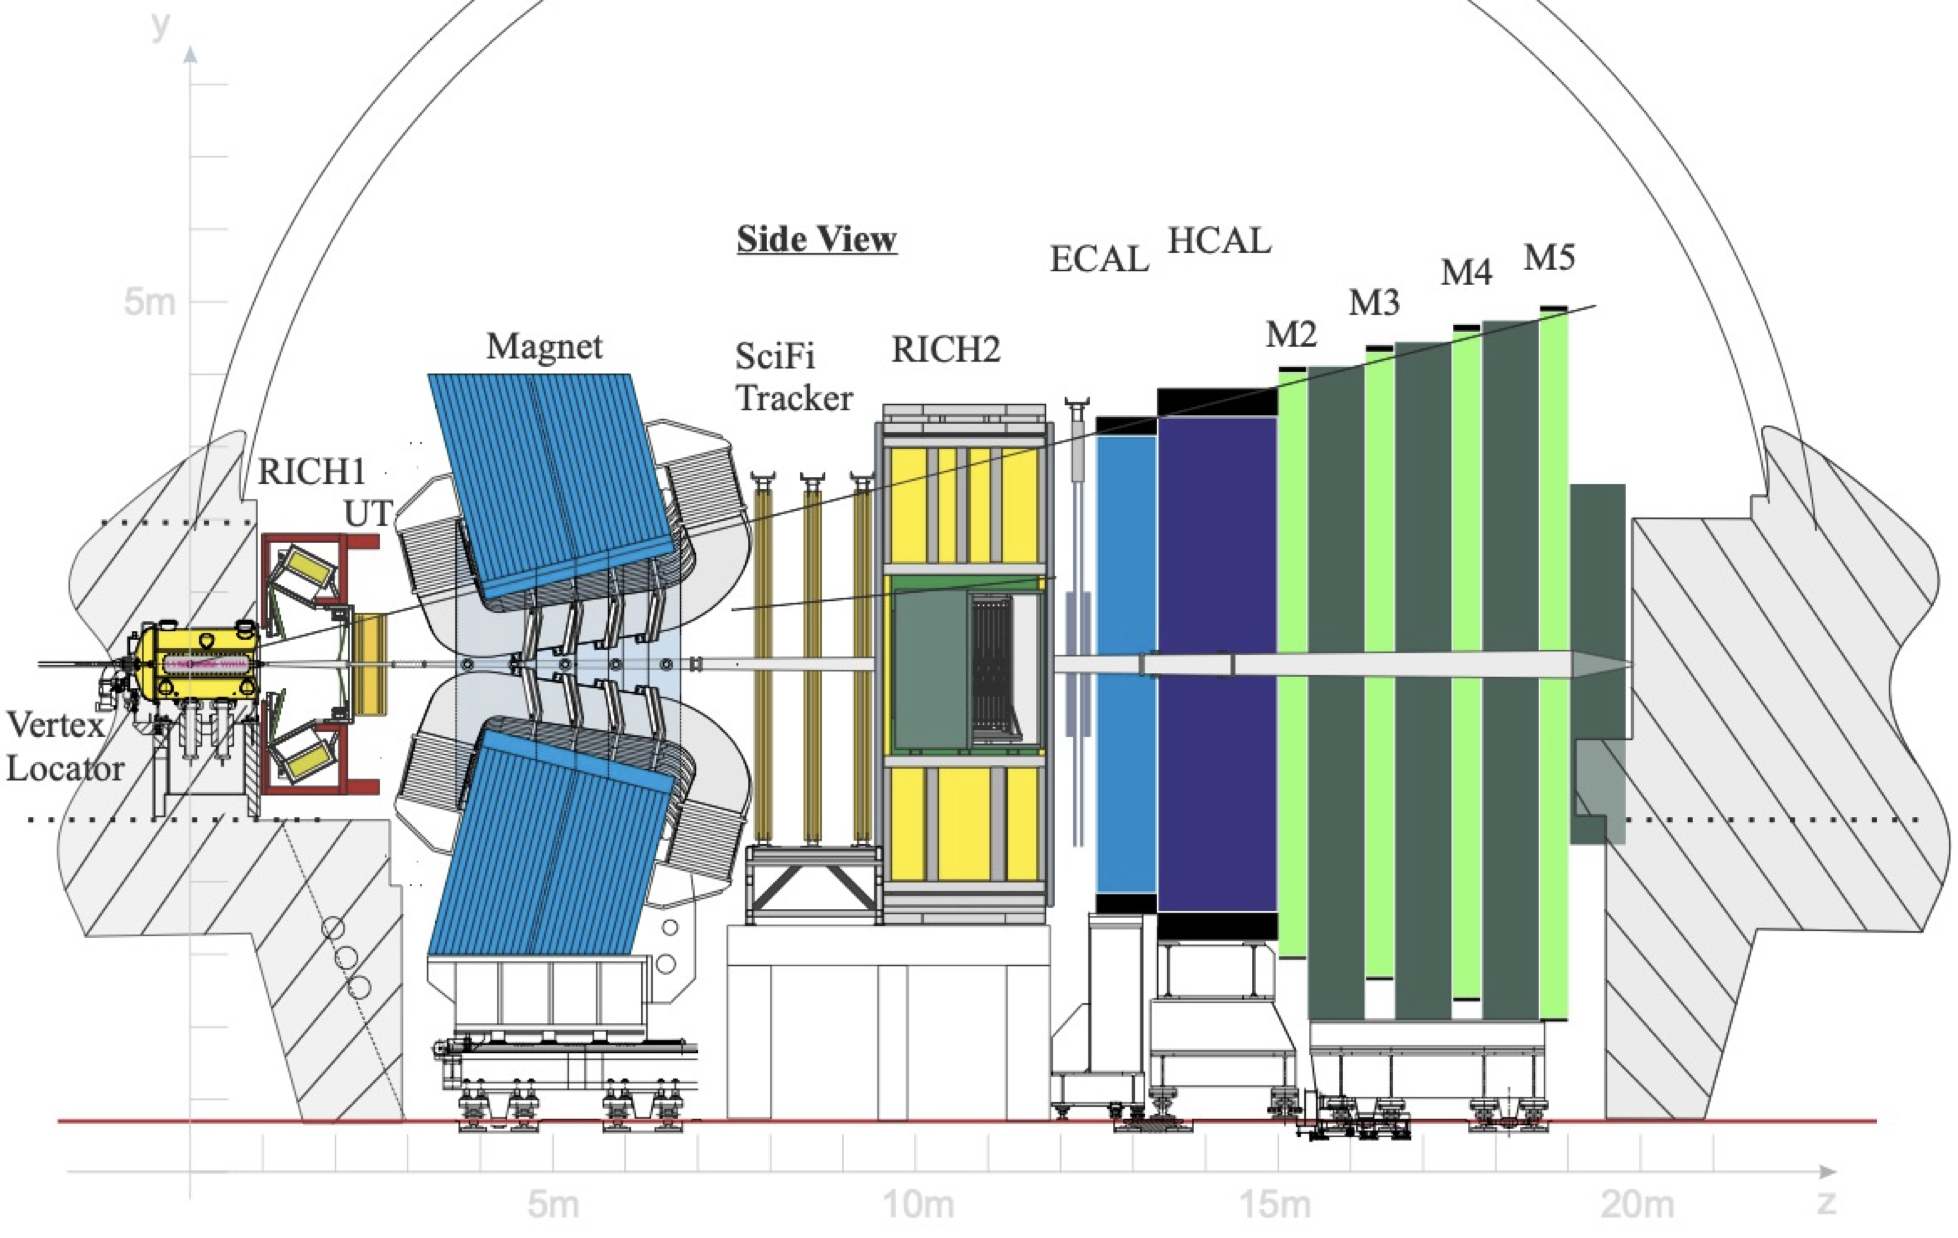
\includegraphics[width=0.9\textwidth]{figures/lhcb_run3.png}
    \caption{Side view of the LHCb detector and its subdetectors during Run 3, taken from \cite{lhcb_upgrade_I}.}
    \label{fig:lhcb_run3}
\end{figure}

Upgrade I introduced major changes to the LHCb experiment. The L0 trigger, which has been removed, lowered signal yields because its transverse energy and momentum thresholds led to the rejection of low-$p_{\text{T}}$, yet physically relevant, events.
The detector and trigger stages are therefore required to process the full crossing rate of $\qty{40}{\mega\hertz}$ provided by the LHC. This is achieved by upgrading the readout electronics, as well as optimizing the HLT algorithms and computing structures. Several subdetectors have been upgraded, removed, or replaced. The PS and SPD detectors, as well as the M1 muon station, were removed, as they were primarily used for the L0 trigger. The tracking system has been fully upgraded and now consists of a silicon-pixel VELO, the Upstream Tracker (UT), and the Scintillating Fiber Tracker (SciFi). The UT, a silicon-based detector, replaces the former TT station. The SciFi tracker comprises three stations, which supersede the previous T1, T2, and T3 stations. Each station contains four detection planes made of scintillating fiber mats, with varying fiber orientations. In addition, the photon detection systems of the RICH detectors have been upgraded.

\section{Impact of Upgrade I on Signal Yields}
\label{sec:lhcb_upgrade_effects}
Since this thesis measures the signal yield $N$ of the rare decay $\Lambda_b^0 \to \Lambda^0 \mu^+ \mu^-$ in both Run 2 and Run 3, it is important to discuss the effects of Upgrade I on this measure. The signal yield is given by
\begin{equation}
    N = 2 \, \mathcal{L} \, \epsilon \, \sigma_{b\bar{b}} \, f_{\Lambda_b^0} \, \mathcal{B}(\Lambda_b^0 \to \Lambda^0 \mu^+ \mu^-) \, \mathcal{B}(\Lambda^0 \to p \pi^-),
    \label{eq:signal_yield}
\end{equation}
where $\mathcal{L}$ is the integrated luminosity, $\sigma_{b\bar{b}}$ the production cross-section of beauty hadrons, $f_{\Lambda_b^0}$ the production fraction of the $\Lambda_b^0$ baryon, $\mathcal{B}$ denotes branching fractions, and $\epsilon$ the total efficiency. $\epsilon$ is the product of several components, including the detector acceptance and efficiencies from all stages of data processing from the trigger and reconstruction to the final signal selection. This analysis is CP-averaged, meaning that both the $\Lambda_b^0$ and $\bar{\Lambda}_b^0$ decays are included. This is reflected by the factor of 2 in \cref{eq:signal_yield}.

The first key difference concerns the total efficiency $\epsilon$, which is influenced by several changes introduced with Upgrade I. Enhancements to the trigger and detector systems affect both the trigger and reconstruction efficiencies, while modifications in the analysis strategy between Run 2 and Run 3 impact the selection efficiency. The second difference is the increased number of visible $pp$ interactions per bunch crossing $\mu$ in Run 3, which can lead to overlapping events and thereby affect the trigger and reconstruction performance. Furthermore, an increase in $\mu$ raises the instantaneous luminosity, yielding a higher integrated luminosity in a shorter time. 